Nous allons utiliser une définition simple de la convexité pour les \ngones, et plus généralement pour les \ncycles. Ceci demande de savoir que, dans un plan orienté, un triangle non dégénéré $ABC$ est dit \focus{orienté positivement} si la condition $\det \big( \vect{AB} , \vect{AC} \big) > 0$ est validée. Dans ce cas, le triangle $BAC$ est orienté négativement, comme cela se vérifie aisément via $\det \big( \vect{AB} , \vect{AB} + \vect{BC} \big)$.
%Pourquoi étudier la convexité des \ncycles? Pour l'existence d'au moins une solution, nous travaillerons dans un ensemble compact, et donc fermé, de \ncycles, or, pour garder des \ngones, nous devrions utiliser des non-égalités, mais ceci nous ferait sortir du cadre fermé qui nous intéresse.


% ----------------------- %


\begin{defi} \label{ncycle-def}
	Un \ncycle\ $\setproba{L} = A_1 A_2 \cdots A_n$ est dit \focus{convexe} si  l'une des alternatives suivantes a lieu.
    %
	\begin{itemize}
		\item $\forall (i, k) \in \ZintervalC{1}{n}^2$,
		$\det \big( \vect{\primeit{A}_i \primeit{A}_{i+1}}, \vect{\primeit{A}_i \primeit{A}_k} \big) \geq 0$.

		\item $\forall (i, k) \in \ZintervalC{1}{n}^2$,
		$\det \big( \vect{\primeit{A}_i \primeit{A}_{i+1}}, \vect{\primeit{A}_i \primeit{A}_k} \big) \leq 0$.
    \end{itemize}
	
	Autrement dit, $\setproba{L} = A_1 A_2 \cdots A_n$ est convexe si l'une des alternatives suivantes a lieu.
    %
	\begin{itemize}
		\item $\forall (i, k) \in \ZintervalC{1}{n}^2$,
		$\primeit{A}_i \primeit{A}_{i+1} \primeit{A}_k$ est soit dégénéré, soit  orienté positivement.

		\item $\forall (i, k) \in \ZintervalC{1}{n}^2$,
		$\primeit{A}_i \primeit{A}_{i+1} \primeit{A}_k$ est soit dégénéré, soit  orienté négativement.
    \end{itemize}
\end{defi}


\begin{remark}
    Voici des exemples pour clarifier le vocabulaire.	
    
    \begin{center}
    	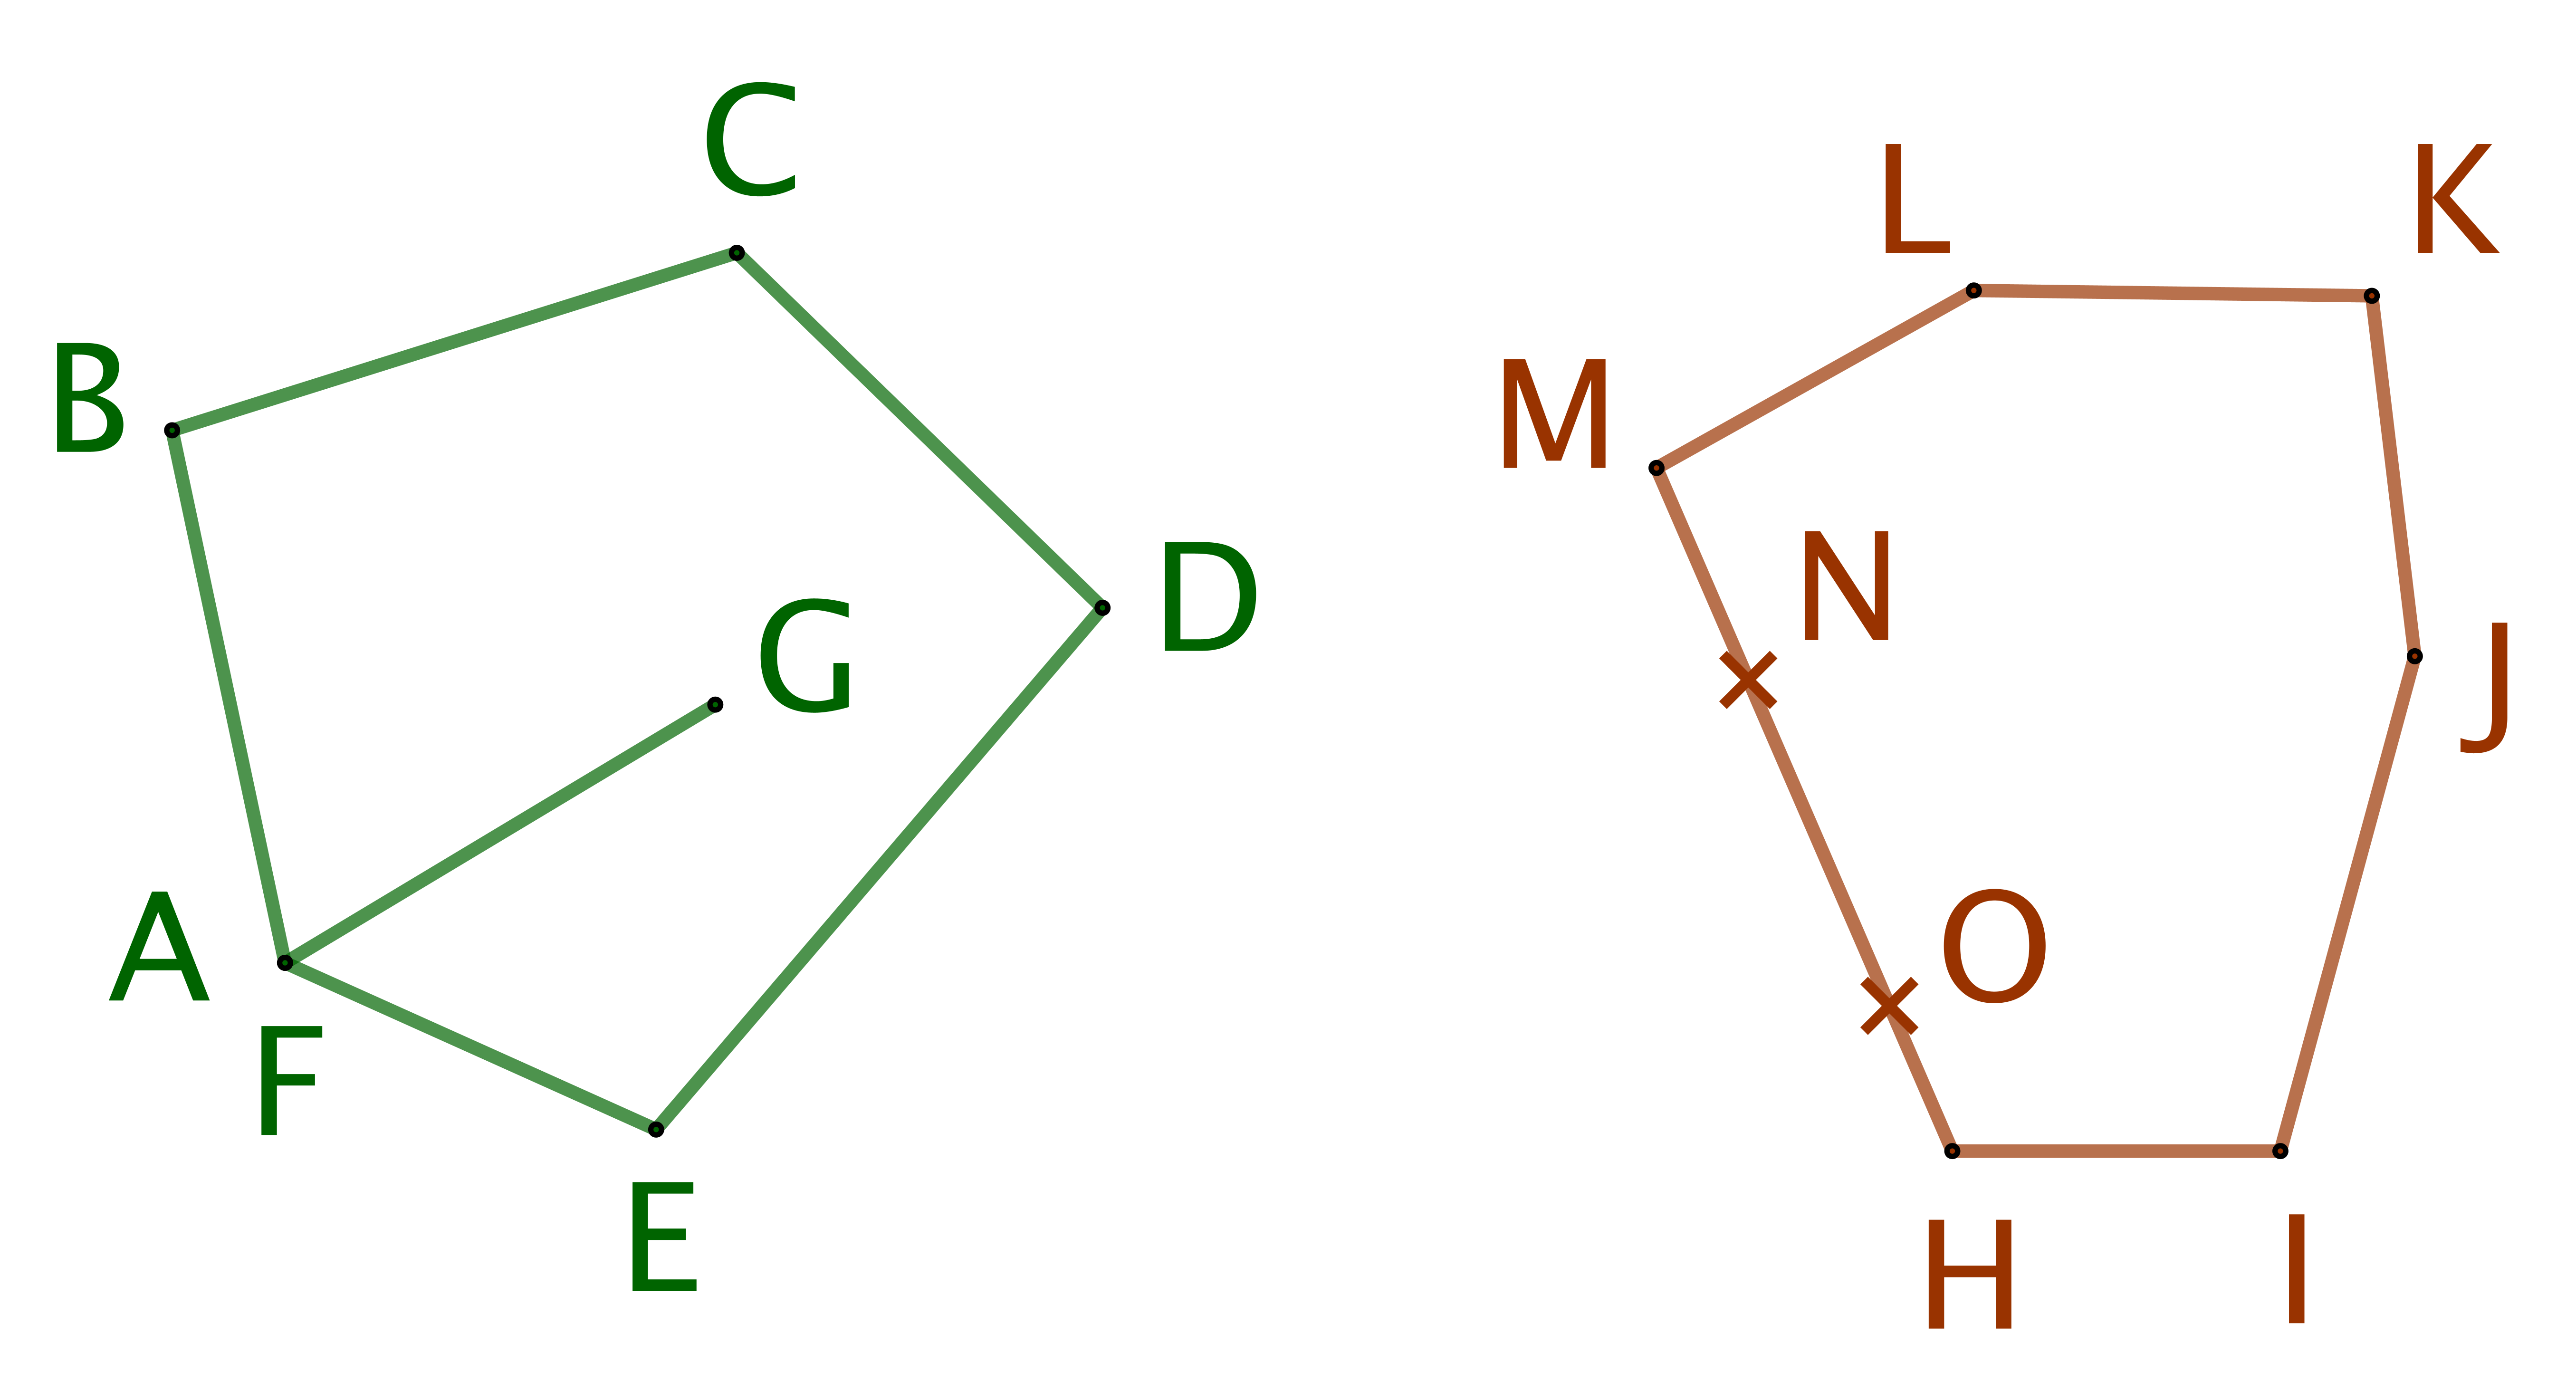
\includegraphics[scale=.3]{degenerated-ncycles.png}
    \end{center}
    
    Le \xcycle{7} non dégénéré $ABCDEFG$ n'est pas convexe, à cause, par exemple, des triangles d'orientations opposées $FGE$ et $FGC$.%
    \footnote{
        $ABCDEFG$ n'est pas un \xgone{7}, car les trois sommets consécutifs $F$, $G$ et $A$ sont alignés.
    }
    Par contre,
    le \xcycle{8} dégénéré $HIJKLMNO$ est convexe, contrairement à $HIJKLMON$, à cause, par exemple, de $MOK$ et $ONK$.%
    \footnote{
         Cet exemple montre que la caractérisation classique de la convexité d'un polygone en terme de demi-espace fermé n'est pas assez précise pour les \ncycles. Ceci est normal, à cause de la possibilité de dégénérescence.
    }
    Enfin,
    $HIJKLM$ est un hexagone convexe.
\end{remark}


% ----------------------- %


\begin{fact} \label{same-hyperplane}
    Soit un \ngone\ $\setproba{P} = A_1 A_2 \cdots A_n$ tel que
    $\forall i \in \ZintervalC{1}{n}$,
    tous les sommets de $\setproba{P}$ sont dans le même demi-plan fermé délimité par la droite $( \primeit{A}_i \primeit{A}_{i+1} )$.
    Plus formellement, nous supposons que
    $\forall (i, j, k) \in \ZintervalC{1}{n}^3$,
    $\det \big( \vect{\primeit{A}_i \primeit{A}_{i+1}}, \vect{\primeit{A}_i \primeit{A}_j} \big)$
    et
    $\det \big( \vect{\primeit{A}_i \primeit{A}_{i+1}}, \vect{\primeit{A}_i \primeit{A}_k} \big)$
    ont le même signe au sens large.
    %
    Bien que nous ne supposions pas, a priori, avoir un signe constant pour des valeurs différentes de $i$, nous pouvons affirmer que $\setproba{P}$ est forcément convexe.
\end{fact}


\begin{proof}
	Le cas des \xgones{3}, c'est-à-dire des triangles non dégénérés, est immédiat.
	Considérons donc $n \geq 4$.
	Comme trois sommets consécutifs de $\setproba{P}$ ne sont jamais alignés, nous avons l'une des deux configurations suivantes dans le plan orienté. 
    
    \begin{multicols}{2}
        \small\itshape\centering
       	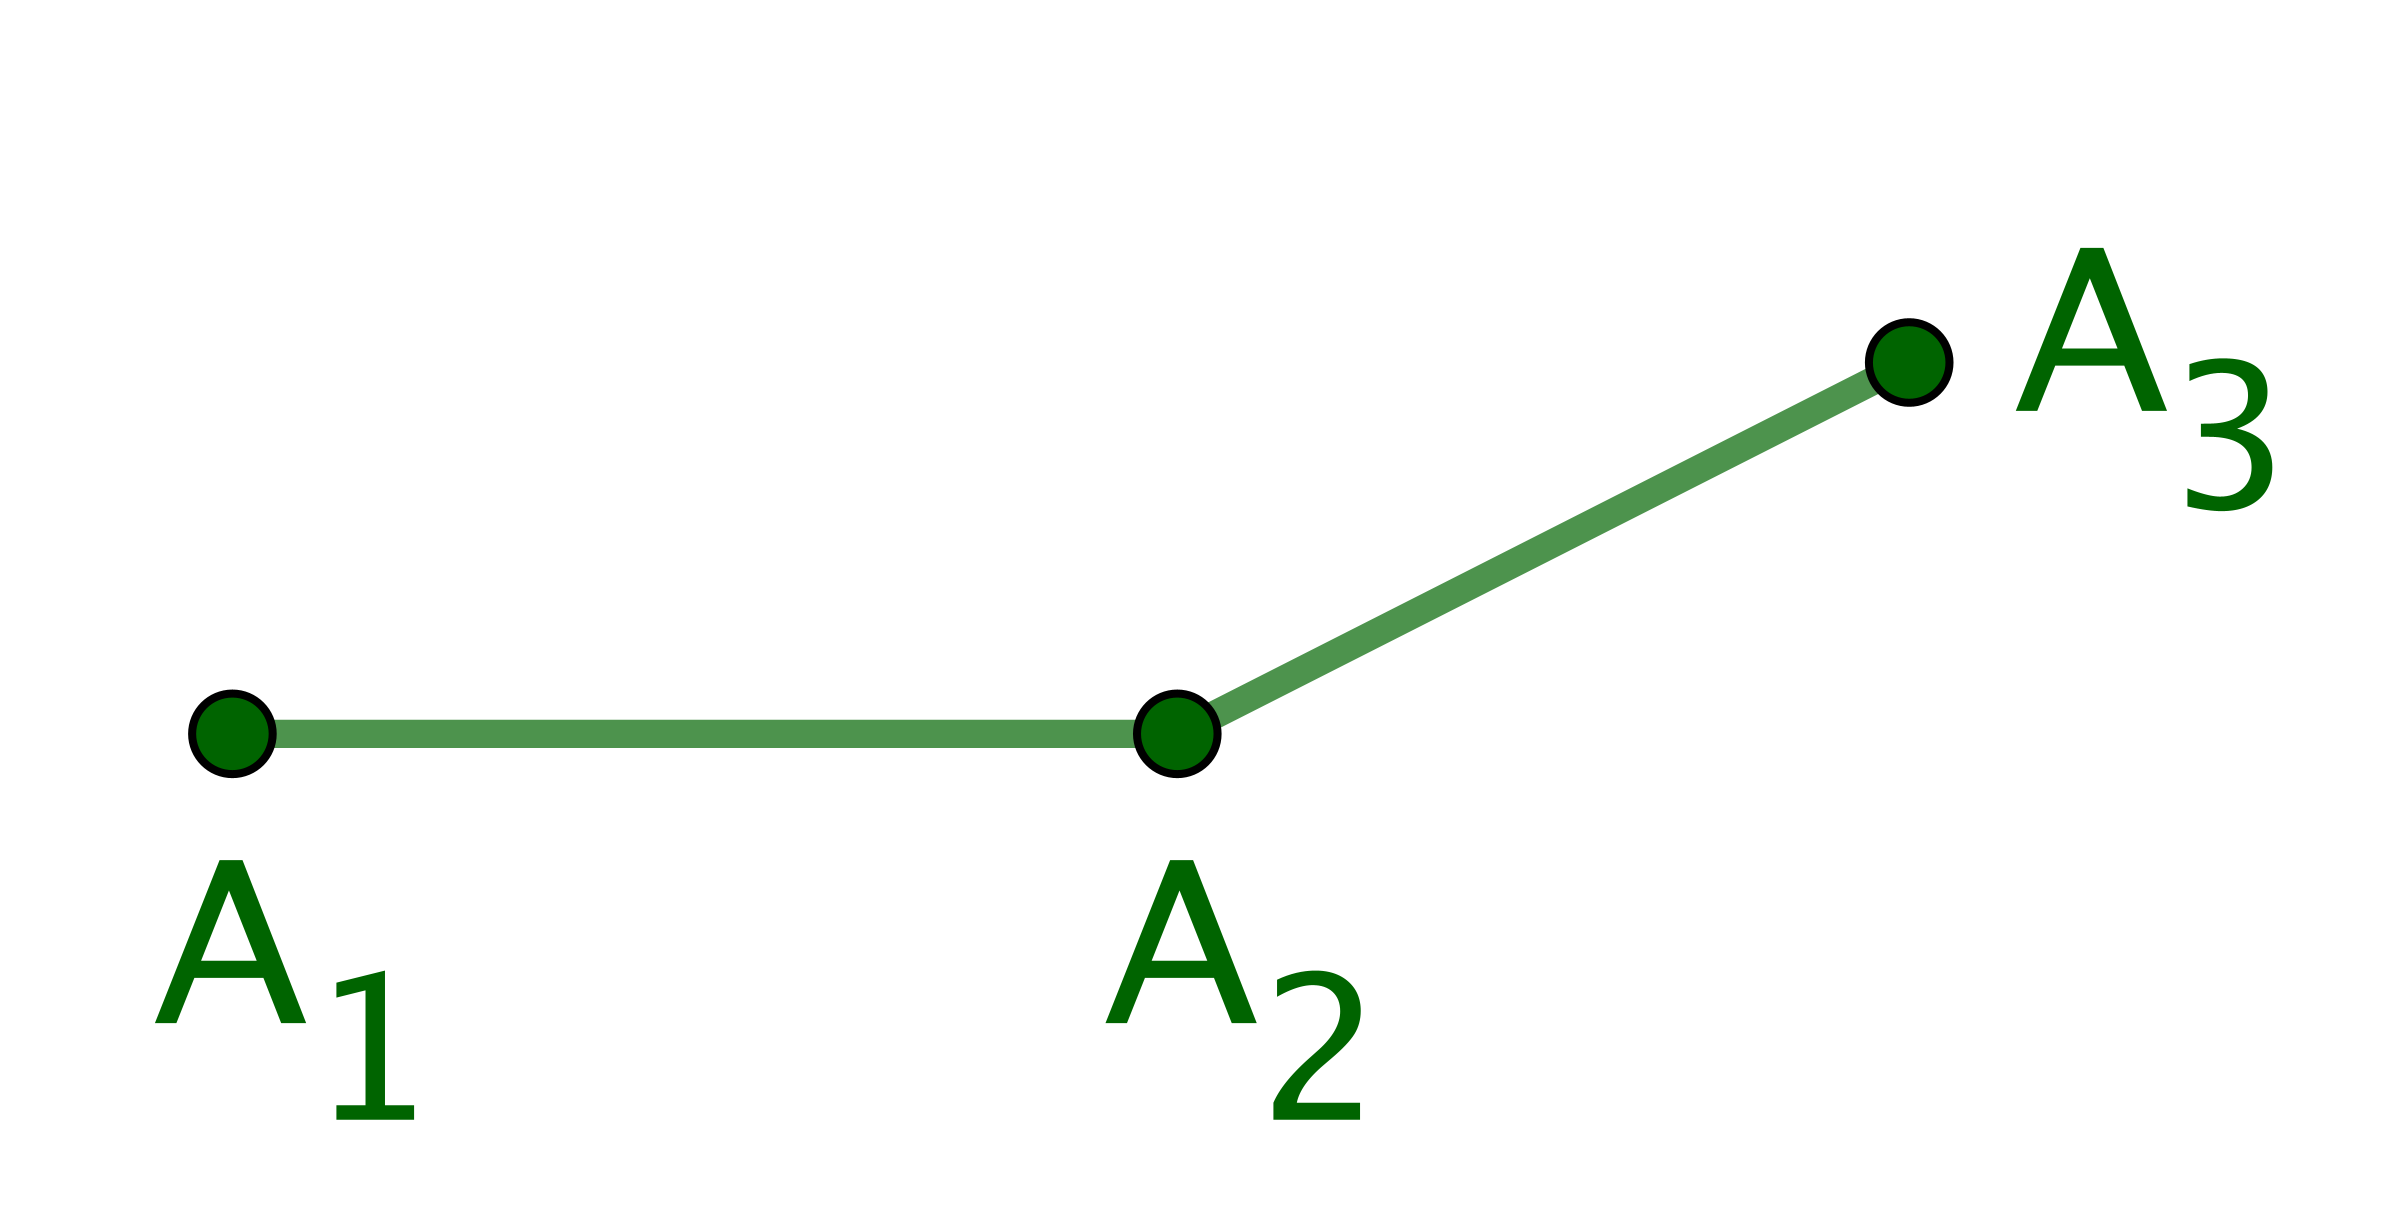
\includegraphics[scale=.4]{det-sign-1.png}
    	    
    	\smallskip
        Cas positif.
        
        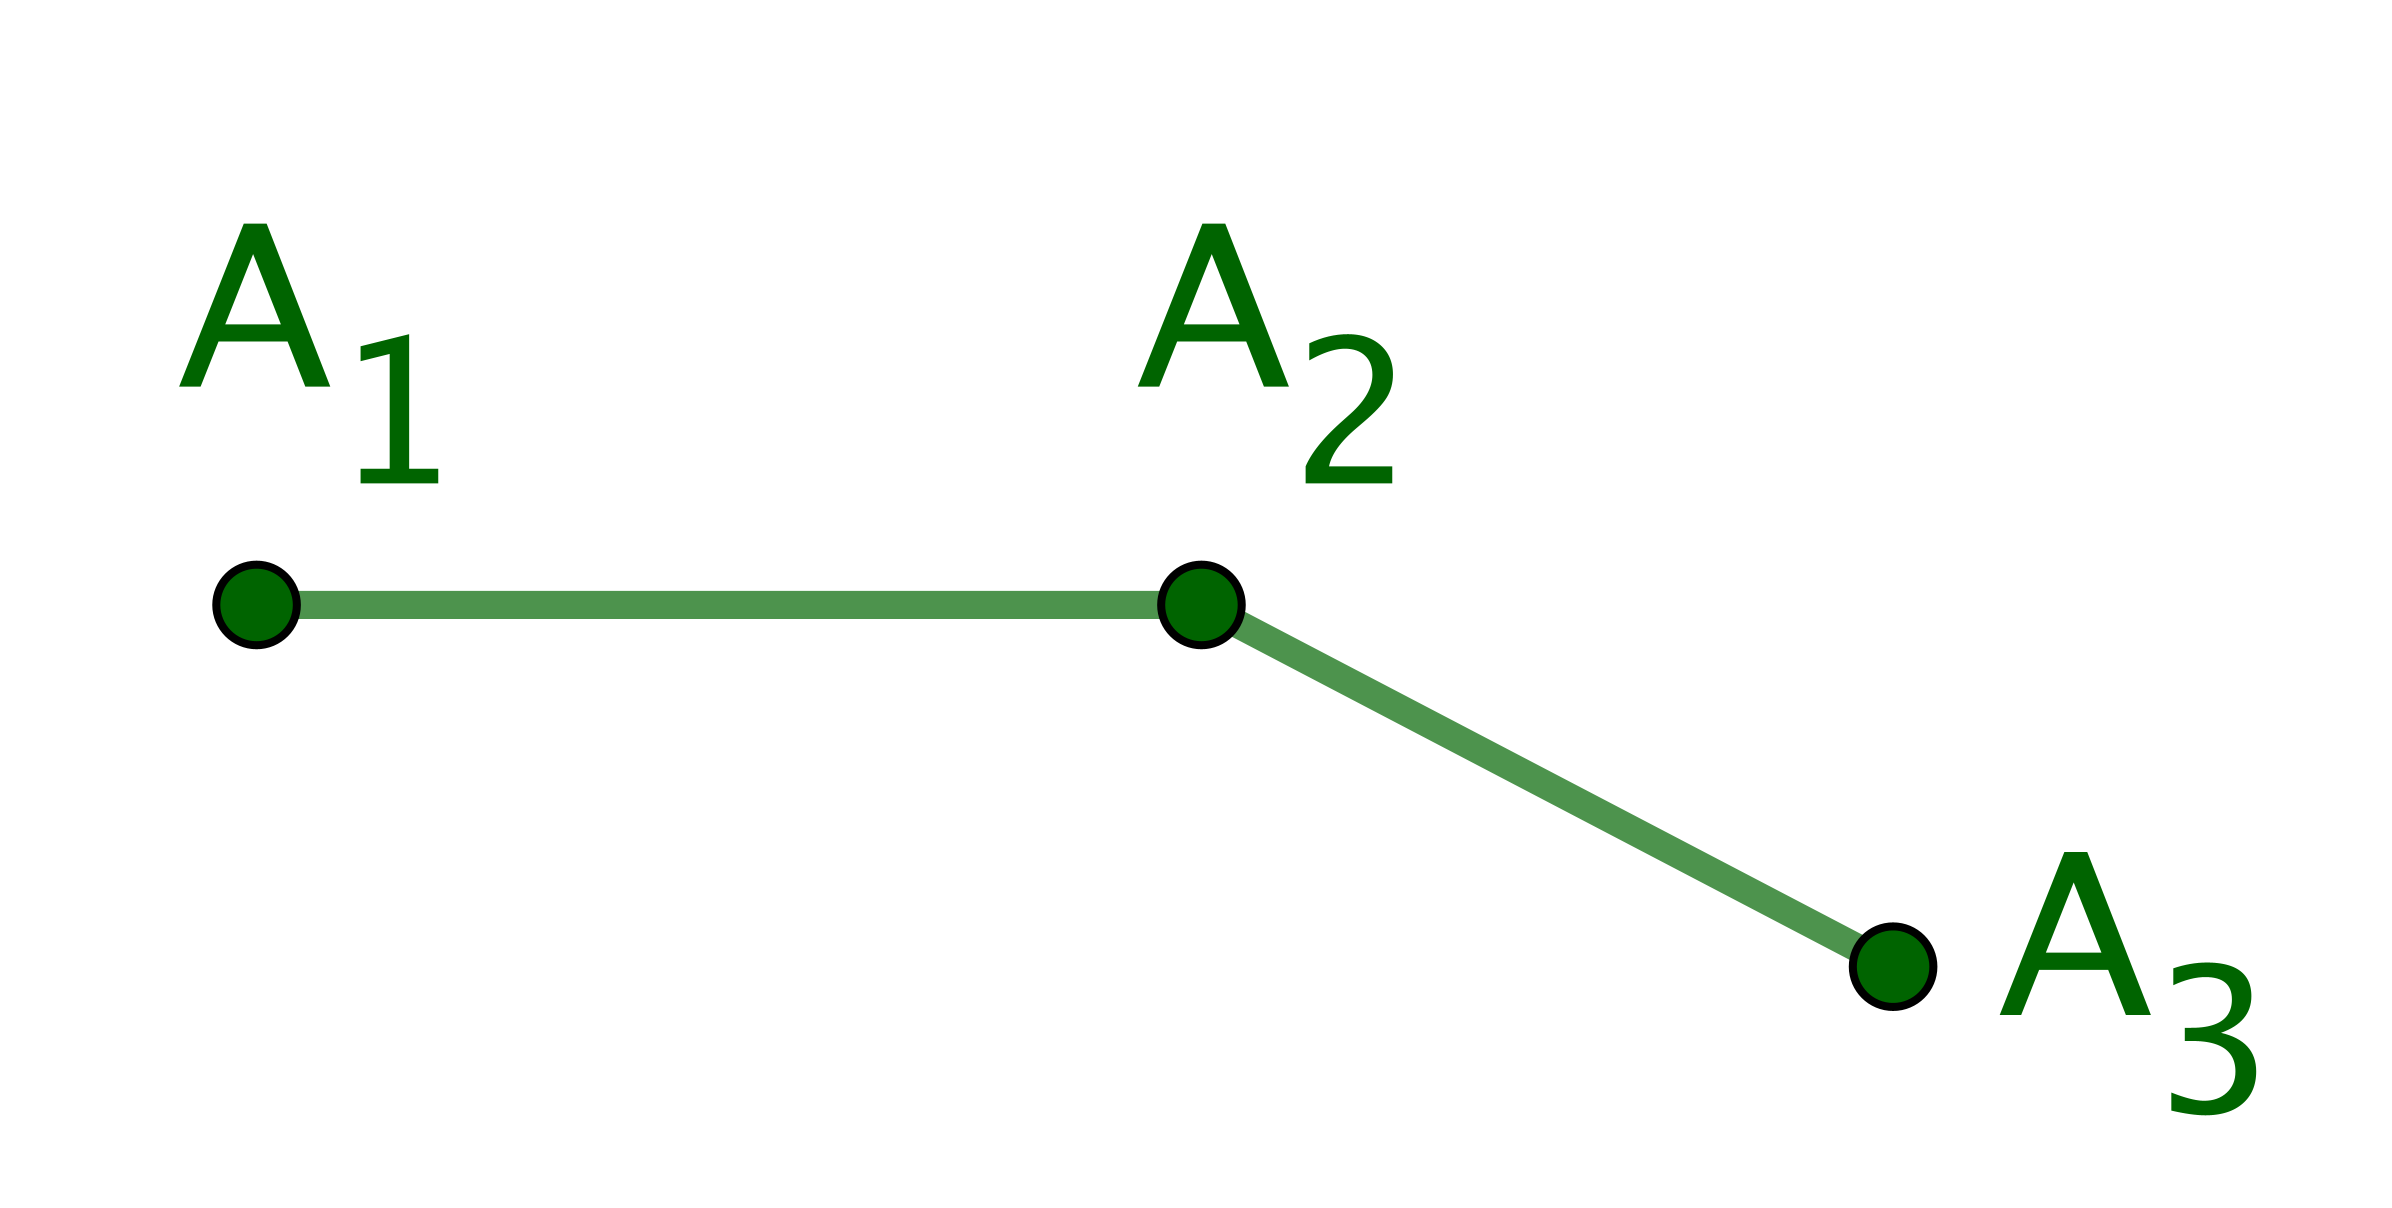
\includegraphics[scale=.4]{det-sign-2.png}
    	    
    	\smallskip
        Cas négatif.
    \end{multicols}


    Par symétrie, nous pouvons juste considérer le cas positif.
	%
	Dès lors,
	$\vect{\primeit{A}_1 \primeit{A}_3} = \vect{\primeit{A}_1 \primeit{A}_2} + \vect{\primeit{A}_2 \primeit{A}_3}$
	et
	$\det \big( \vect{\primeit{A}_1 \primeit{A}_2}, \vect{\primeit{A}_1 \primeit{A}_3} \big) > 0$
    nous donnent
	$\det \big( \vect{\primeit{A}_2 \primeit{A}_3}, \vect{\primeit{A}_2 \primeit{A}_1} \big) > 0$.
	Or, $A_2$, $A_3$ et $A_4$ ne sont pas alignés, et de plus $A_1$ et $A_4$ sont du même côté de la droite $(A_2 A_3)$, au sens large,
	donc nous avons
	$\det \big( \vect{\primeit{A}_2 \primeit{A}_3}, \vect{\primeit{A}_2 \primeit{A}_4} \big) > 0$.
	%
	En continuant de proche en proche, nous arrivons à
	$\det \big( \vect{\primeit{A}_i \primeit{A}_{i+1}}, \vect{\primeit{A}_i \primeit{A}_{i+2}} \big) > 0$
	pour $i \in \ZintervalC{1}{n}$ quelconque.
	%
	Comme tous les sommets de $\setproba{P}$ sont du même côté de la droite $( \primeit{A}_i \primeit{A}_{i+1} )$, ou sur elle,
	nous obtenons alors
	$\det \big( \vect{\primeit{A}_i \primeit{A}_{i+1}}, \vect{\primeit{A}_i \primeit{A}_k} \big) \geq 0$
	pour $(i, k) \in \ZintervalC{1}{n}^2$.
	Ceci établit la convexité de $\setproba{P}$.
\end{proof}


% ----------------------- %


\begin{remark}
    La définition standard d'un \ngone\ convexe $\setproba{P}$ dit qu'il doit être tel que pour toute paire de points $M$ et $N$ de la surface fermée bornée $\setproba{S}$ créée par $\setproba{P}$, le segment $[MN]$ est dans cette surface.
    Grâce au fait \ref{same-hyperplane} précédent, la surface $\setproba{S}$ peut se définir comme étant l'ensemble des points $M$ du même côté de la droite $( \primeit{A}_i \primeit{A}_{i+1} )$ que le sommet $\primeit{A}_{i+2}$.
    Il devient facile de démontrer que notre définition de la convexité implique celle usuelle. 
\end{remark}
